% Define the page style
\fancypagestyle{chapterstyle}{
   \fancyhead[L]{\nouppercase{\rightmark}}
   \fancyhead[R]{Projet de fin d'etudes 2023-2024}
   \fancyfoot[C]{\vspace{20pt}\thepage} % Adjust the vertical space here
   \setlength{\headheight}{20pt}
   \setlength{\footskip}{30pt} % Adjust the value as needed
}

\chapter{Contexte Général}
\pagestyle{chapterstyle}
Ce premier chapitre a pour objectif de présenter
l’organisme d’accueil, son historique, ses objectifs
et ses activités. Il fournira également une 
description du contexte du projet, en mettant
en évidence le problème qu’il vise à résoudre, 
les attentes associées, ainsi que la gestion et 
la planification de sa mise en œuvre.



\newpage
\vspace{1cm}
\section{Introduction}
% \vspace{1cm}

% Dans ce chapitre nous allons commencer par une présentation de l’organisme d’accueil, 
% son histoire, ses services et bien d’autres informations, 
% puis nous aborderons la méthodologie de travail pendant 
% les quatre mois de stage et finalement la manière dont nous avons géré notre projet.

Le premier chapitre vise à introduire le projet de manière générale. 
Il est divisé en trois parties principales, chacune ayant 
plusieurs sections. La première partie offre une courte présentation 
de 4D Logiciels Maroc, en expliquant son architecture, ses missions 
ainsi que le groupe 4D et ses produits. La deuxième partie situe 
le projet dans son contexte en décrivant son cadre général, 
la problématique à la base de sa création et les différents 
objectifs visés. Enfin, la dernière partie détaille la méthode 
de conduite de projet choisie.


%%%%%%%%%%%%%%%%%%%% SECTION 2 %%%%%%%%%%%%%%%%%%%%%%%

\section{Présentation de l’organisme d’accueil}

Fondée en 1984 par Laurent Ribardière, 4D logiciel est une entreprise de conseil et de
développement de logiciels dans le domaine des systèmes d’informations, de l’organisation
et de l’informatique dont le siège social se situe à Clichy (Île-de-France).
\newline

Laurent Ribardière a créé 4D avec une seule ambition : simplifier la création des
applications professionnelles pour les entreprises grâce à une base de données relationnelles
entièrement graphique.
\newline

4D est devenue ainsi l’un des premiers éditeurs de logiciels français avec un rayonnement international grâce à sa présence sur les cinq continents et des filiales dans plus de
dix pays dont le Maroc (4D Logiciels Maroc).
\newline

Le succès de 4D vient de sa capacité à répondre aux enjeux de son époque, grâce à
une plateforme évolutive, simplifiant la création d’expériences clients réussies sur mobile,
web, desktop.


\begin{figure}[h]
    \centering
    
\includegraphics[scale=1.5]{Images/logo-4d.jpg} % Replace with the actual filename of the IBM logo image
    \caption{Logo 4D}
    \label{fig:Logo4D}
\end{figure}



%%%%%%%%%%%%%%%%%%%% subsection 1 %%%%%%%%%%%%%%%%%%%%%%%

\subsection{Histoire de 4D}

L’entreprise 4D Logiciels, une entreprise faisant partie du marché de l’édition logicielle
dont le siège est situé en France.
\newline
\newline
\newline
\newline


\begin{figure}[h]
    \centering
    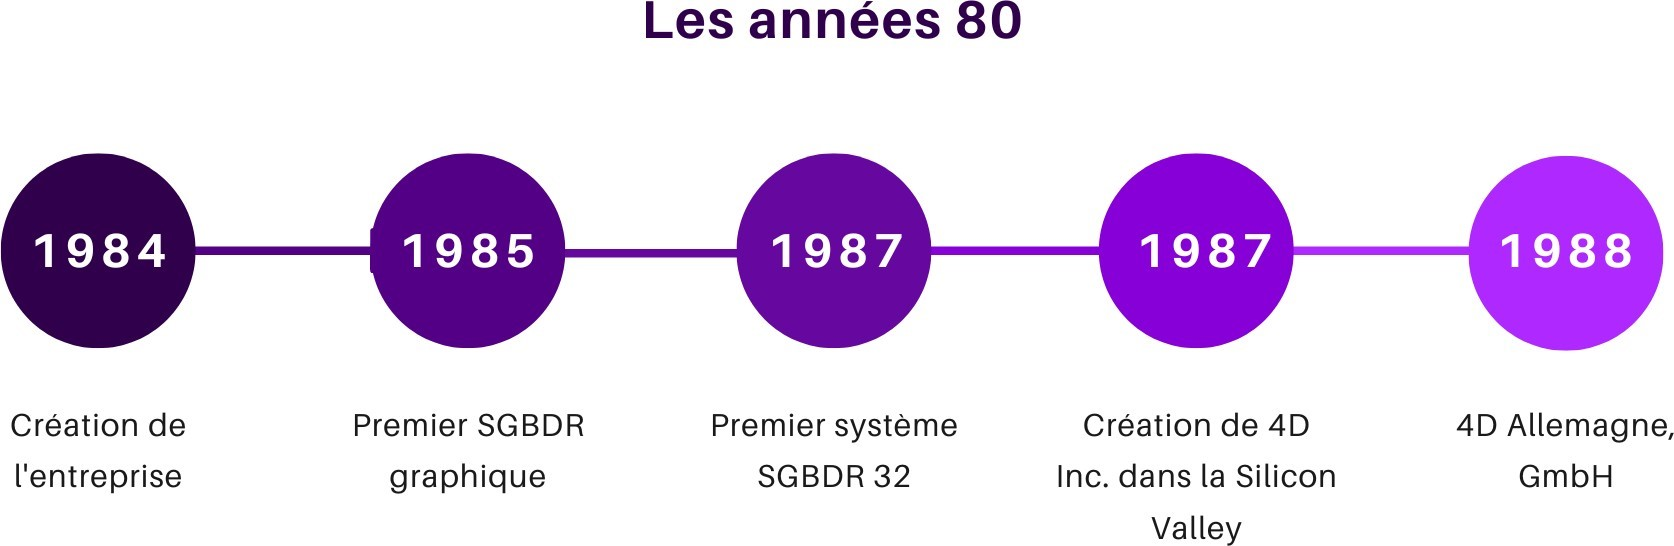
\includegraphics[scale=0.3]{Images/80.jpg} % Replace with the actual filename of the IBM logo image
    \caption{Les années 80}
    \label{fig:Histoire80}
\end{figure}


Crée en 1984, 4D Logiciels est reconnu par ses outils de développement innovants permettant de créer des solutions professionnelles performantes et fiables au service des entreprises.
En 1987, 4D Logiciels propose le premier système de gestion de base de données relationnel fonctionnant sur un système 32-bits, puis conserve sa place de leader en offrant le premier :
\begin{itemize}
    \item • Client-serveur intégré.
    \item • Serveur web intégré.
    \item • Système de partage d’applications dynamique intégré.
\end{itemize}
\vspace{1cm}

\begin{figure}[h]
    \centering
    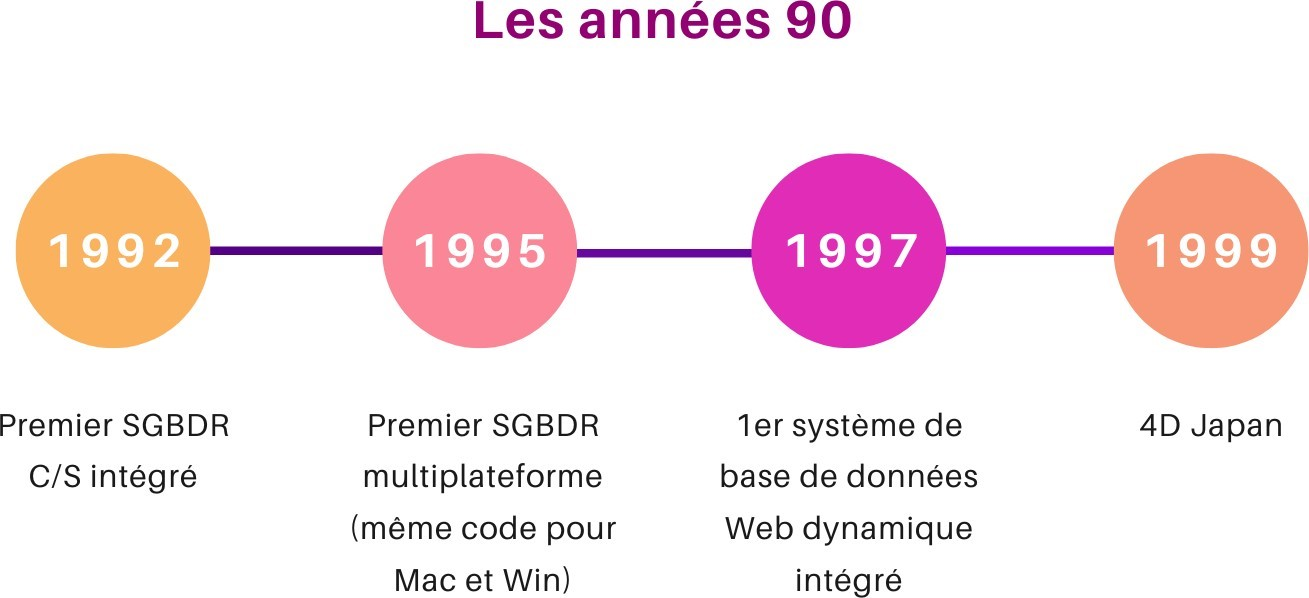
\includegraphics[scale=0.3]{Images/90.jpg} % Replace with the actual filename of the IBM logo image
    \caption{Les années 90}
    \label{fig:Histoire90}
\end{figure}
% \vspace{lcm}

En 1997, 4D décide de s’investir dans le Web en donnant lieu 
à un serveur Web dynamique. Ce qui aide les développeurs à servir
à la fois des applications client-serveur et des applications
Web sans modifier le code. 4D conserve par la suite ce produit 
en lançant à chaque fois des nouvelles versions.
\vspace{6cm}

\begin{figure}[h]
    \centering
    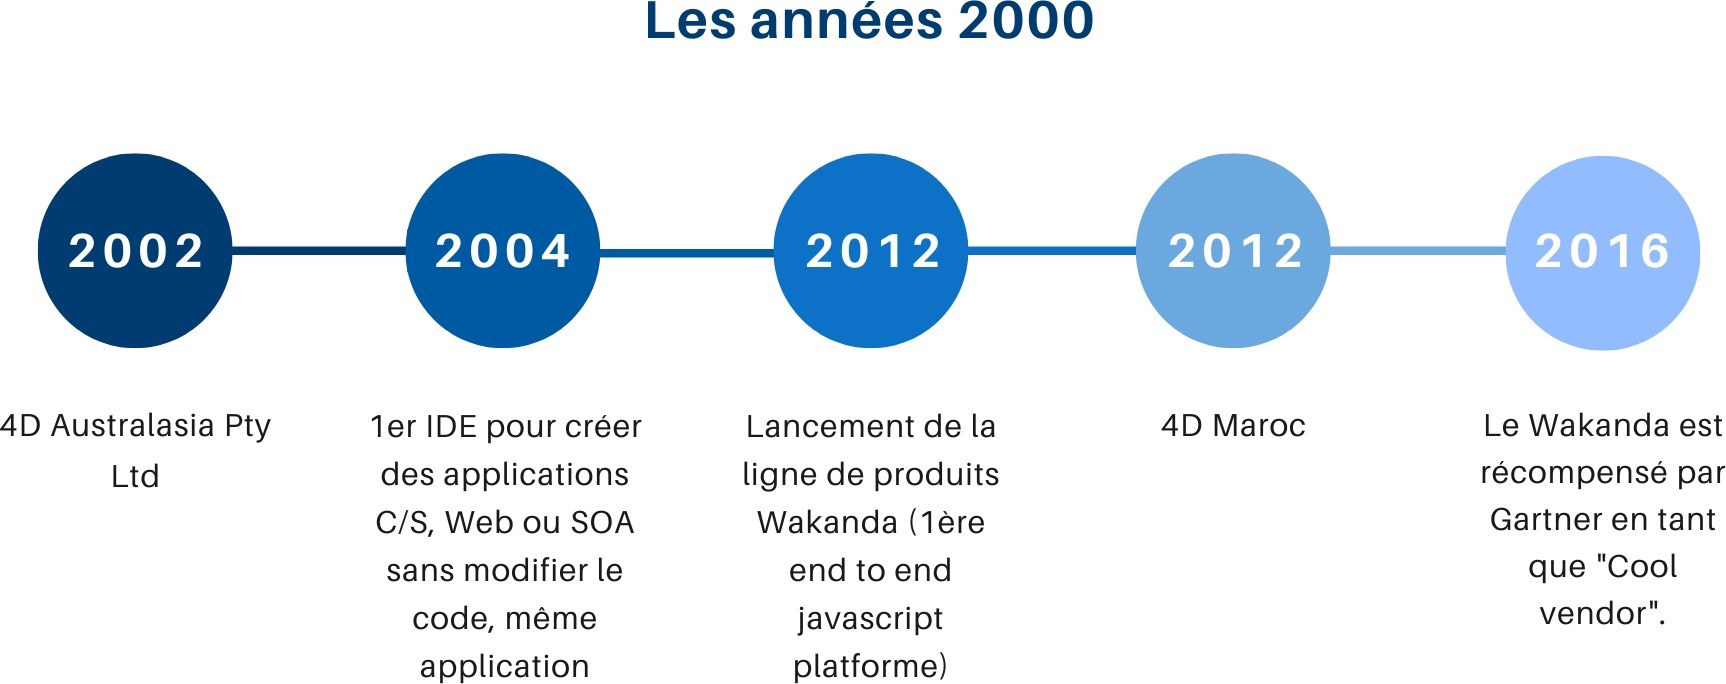
\includegraphics[scale=0.3]{Images/20.jpg} % Replace with the actual filename of the IBM logo image
    \caption{Les années 2000}
    \label{fig:Histoire90}
\end{figure}

La version 4D 2004 se lance en tant qu’un produit permettant aux développeurs 
de créer à la fois des applications autonomes, client-serveur, Web, 
ainsi que des applications orientées Services (SOA) sans rajouter 
aucun changement au niveau du code.
Plus récemment, 4D dispose d’une plateforme de développement 
en JavaScript qui facilite la création des applications 
professionnelles en utilisant la gamme de produits Wakanda.


%%%%%%%%%%%%%%%%%%%% subsection 2 %%%%%%%%%%%%%%%%%%%%%%%

\subsection{Le Langage 4D}

4D est une plateforme de développement productive qui permet aux clients
 de se concentrer sur leur modèle de données et les règles 
 et spécificités de leur métier [1].
 Le langage 4D prend en charge l’exécution native 
 de leur code applicatif sous macOS et Windows. 
 4D Serveur exécute leurs applications simultanément sur les postes de travail
/ clients mobiles et sur le Web. Ils peuvent déployer des applications 
entièrement personnalisées sous leur propre marque.
 4D est un système de gestion de base de données 
 relationnelle disposant d’un langage de programmation 
 de la quatrième génération.
\newline

Environnement de développement intégré, 4D intègre :
\begin{itemize}
    \item un compilateur
    \item un débogueur
    \item un système de sauvegarde et de réplication
    \item un serveur Web
    \item un serveur et client de services web
\end{itemize}

\begin{figure}[h]
    \centering
    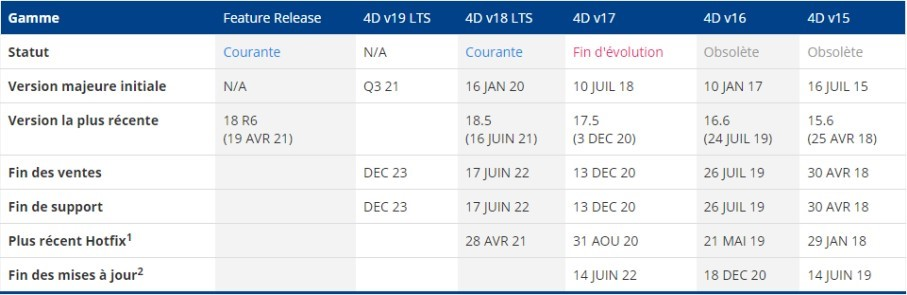
\includegraphics[scale=0.7]{Images/versions.jpg} % Replace with the actual filename of the IBM logo image
    \caption{Anciennes versions de 4D}
    \label{fig:AncienneVersions}
\end{figure}

\vspace{6cm}
4D v18 marque un véritable tournant dans l’histoire de 4D. Cette version propose non seulement de
multiples nouvelles fonctionnalités, mais aussi l’amélioration de fonctions existantes. Elle introduit la gestion de version pour changer 
la façon dont les équipes collaborent. Le format texte des bases projets permet désormais de tirer pleinement parti des systèmes de gestion de version
(par exemple, Git, SVN, etc.). Autre fonctionnalité qui fait ses débuts dans cette nouvelle version : une solution intégrée de chiffrement des données, 
offrant en un seul clic une sécurité maximum aux données des clients. Ces outils de chiffrement sont basés sur l’un des algorithmes les plus sûrs : 
Advanced Encryption Standard (AES). ORDA (Object Relational Data Access), la technologie révolutionnaire d’accès et de présentation 
des données, apporte également son lot de nouvelles fonction- nalités, telles que le Datastore distant, ouvrant de nouvelles perspectives et optimisant les 
performances du client/serveur. Les applications métiers peuvent facilement être dé- ployées sur des appareils mobiles avec 4D for iOS, une solution 
entièrement intégrée à 4D. De plus, 4D Write Pro, outil de PAO intégré à 4D, poursuit sa montée en puissance, le langage de programmation 4D s’enrichit et apporte de nouvelles commandes destinées à améliorer l’expérience de développement.
\newline

La dernière version du produit 4D, 4D v19 R8, est une version encore plus améliorée qui offre de nouvelles 
fonctionnalités. Cette version est particulièrement intéressante pour les développeurs et les utilisateurs de 4D,
car elle leur permet de bénéficier de performances accrues et d’une expérience utilisateur améliorée.
En effet, les améliorations apportées à cette version ont été conçues pour répondre aux besoins des utilisateurs de manière plus efficace.
\newline

La version 4D v20 est actuellement en version beta, ce qui signifie 
qu’elle est encore en phase de test. Cette version n’est pas encore 
disponible pour une utilisation générale, mais elle est plutôt réservée 
à un groupe restreint de testeurs qui vont l’évaluer et signaler 
les éventuels problèmes ou bugs. Cette phase de test permet à l’équipe 
de développement de recueillir des commentaires et des suggestions de la part 
des testeurs afin d’améliorer la qualité du logiciel avant sa sortie officielle. 
En bref, la version 4D v20 est en mode testing pour s’assurer qu’elle est stable et 
fiable avant d’être rendue disponible pour le grand public.

\vspace{0.5cm}

\begin{figure}[h]
    \centering
    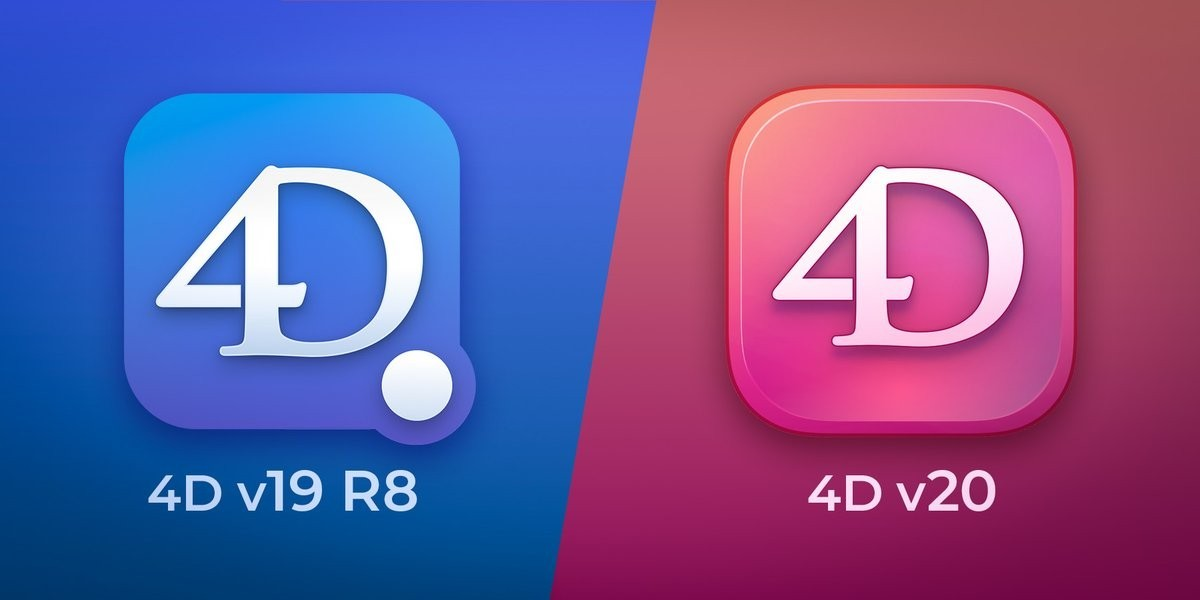
\includegraphics[scale=0.3]{Images/v19v20.jpg} % Replace with the actual filename of the IBM logo image
    \caption{les deux nouvelles versions de 4D}
    \label{fig:v19v20}
\end{figure}


%%%%%%%%%%%%%%%%%%%% subsection 3 %%%%%%%%%%%%%%%%%%%%%%%

\subsection{La structure du groupe 4D}
Acteur dans le métier de l’édition de logiciel, la société
4D développe et commercialise depuis plus de trente 
ans à travers le monde, une plateforme logicielle 
intégrée qui accélère et simplifie le développement
et le déploiement des applications métiers des clients finaux.
Le groupe 4D est composé d’un siège social situé en France, 
et de cinq filiales situées aux États-Unis, en Allemagne, 
en Australie, au Japon, et au Marocj[1]. À l’écoute permanente 
de leurs besoins et des évolutions technologiques, 
la société propose une aven- ture passionnante dans un 
contexte multiculturel à travers ses différentes implantations 
à l’international (Sydney, Tokyo, San José, Munich, Rabat).

\vspace{1cm}

\begin{figure}[h]
    \centering
    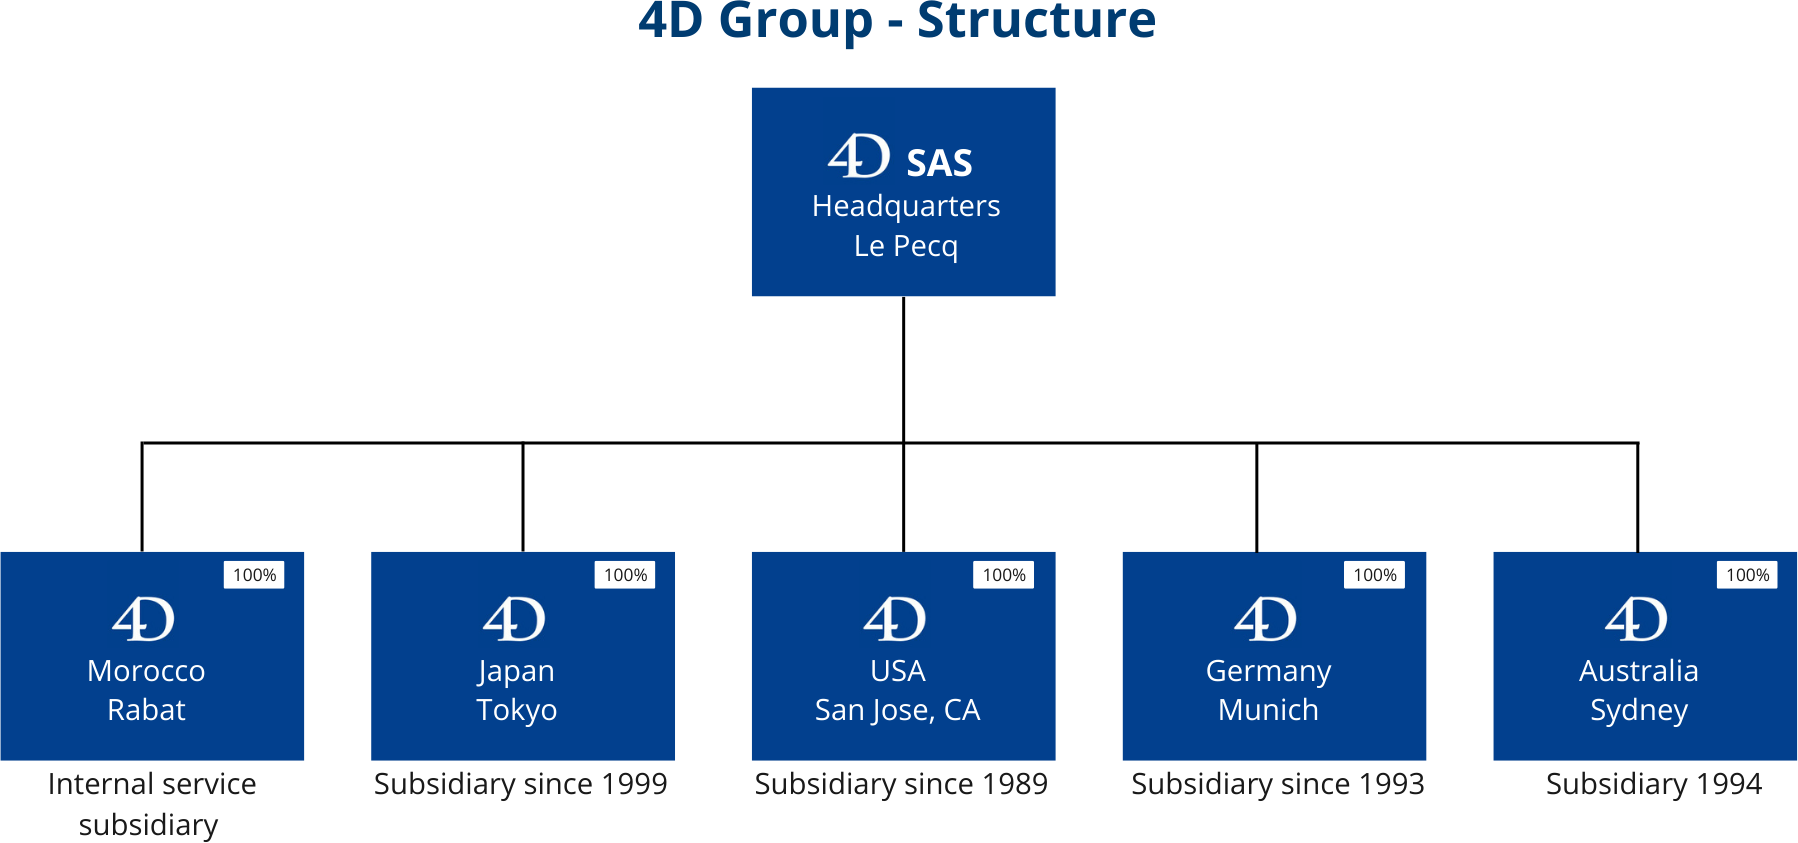
\includegraphics[scale=0.35]{Images/groupe.png} % Replace with the actual filename of the IBM logo image
    \caption{Le groupe 4D dans le monde}
    \label{fig:groupe}
\end{figure}

Comme toute société renommée, 4D recourt à ses différents partenaires 
pour un rendu meilleur et un niveau d’expertise plus crédible. 4D connaît aussi 
une présence internatio- nale grâce à ses partenaires et ses distributeurs éparpillés 
dans le monde, comme montre la figure suivante :

\begin{figure}[h]
    \centering
    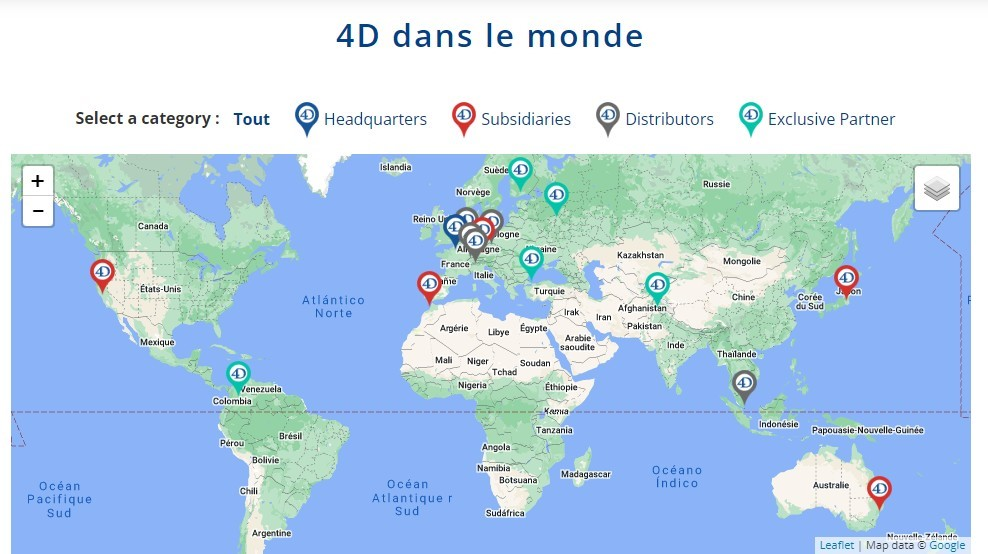
\includegraphics[scale=0.6]{Images/carte.jpg} % Replace with the actual filename of the IBM logo image
    \caption{Les points de présence des partenaires et des distributeurs de 4D}
    \label{fig:carte}
\end{figure}

La figure ci-dessous montre la direction générale de l’entreprise 4D logiciels :

\begin{figure}[h]
    \centering
    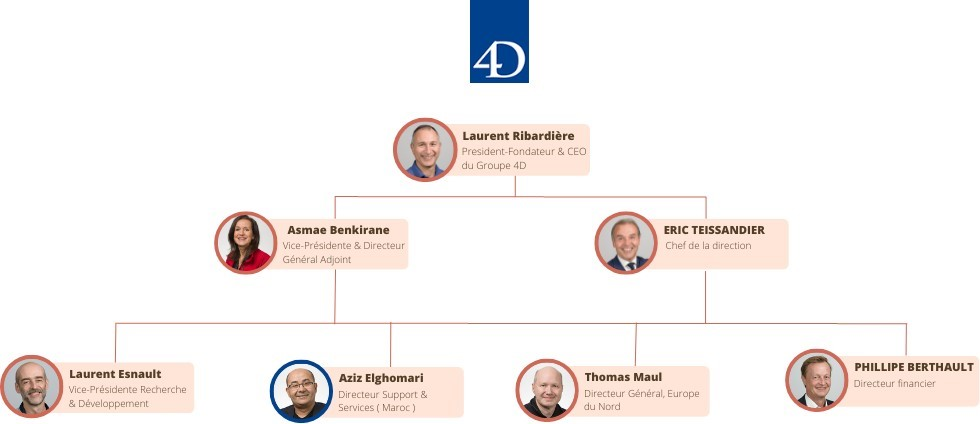
\includegraphics[scale=0.6]{Images/direction.jpg} % Replace with the actual filename of the IBM logo image
    \caption{La Direction Générale de 4D}
    \label{fig:direction}
\end{figure}

%%%%%%%%%%%%%%%%%%%% subsection 4 %%%%%%%%%%%%%%%%%%%%%%%
\subsection{Les domaines Métiers et les clients 4D}
4D intervient dans une diversité de domaines, comme 
la santé, l’éducation, l’adminis- tration, la gouvernance, 
et les télécommunications. La figure 1.6 montre le pourcentage 
qu’occupe chaque domaine dans son activité.

\begin{figure}[h]
    \centering
    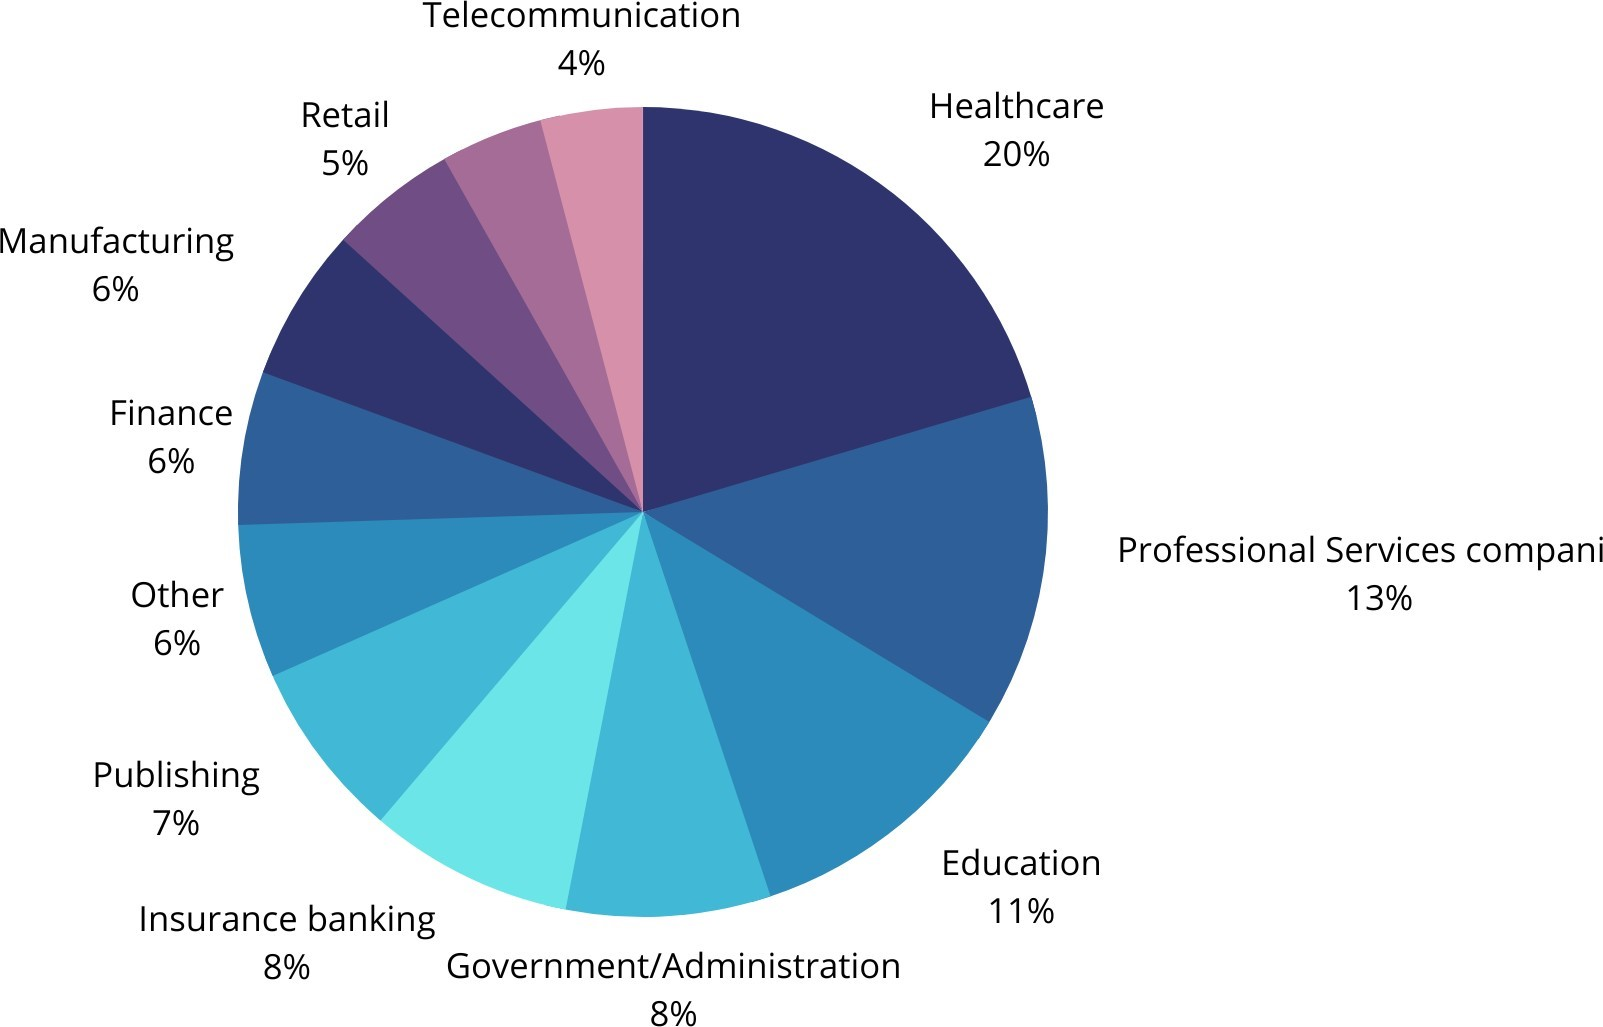
\includegraphics[scale=0.3]{Images/domaineMetier.jpg} % Replace with the actual filename of the IBM logo image
    \caption{Les domaines métiers de 4D en pourcentage}
    \label{fig:domaineMetier}
\end{figure}


%%%%%%%%%%%%%%%%%%%% SECTION 3 %%%%%%%%%%%%%%%%%%%%%%%

\section{Présentation du projet}
\subsection{Cadre du projet}
Dans un environnement où la concurrence pour attirer les meilleurs talents
 est de plus en plus intense, les entreprises doivent disposer d'outils 
 efficaces pour gérer leur processus de recrutement. Actuellement, 
 4D Logiciels utilise un système disparate et manuel pour le recrutement, 
 ce qui entraîne des inefficacités et des pertes de temps. Cette situation 
 rend difficile la gestion des candidatures, la traçabilité des étapes de 
 recrutement, et la communication entre les recruteurs et les candidats.

Afin de renforcer le niveau de ses collaborateurs, 4D Logiciels souhaite 
simplifier et moderniser son processus de recrutement. L'objectif est de passer 
d'un système essentiellement manuel à une solution plus intégrée et automatisée, 
permettant d'améliorer l'efficacité, de réduire les délais de recrutement, 
et d'offrir une meilleure expérience aux candidats.

\subsection{Problématique}
L'entreprise 4D Logiciels est confrontée à une gestion inefficace
 de ses processus de recrutement, notamment lorsqu'elle publie 
 des offres d'emploi et ouvre des opportunités de stage annuelles.
4D Logiciels reçoit un grand nombre de candidatures non triées,
provenant de divers domaines, ce qui rend difficile la
sélection des candidats les plus appropriés. Les méthodes 
traditionnelles utilisées, telles que les emails, les tableurs 
et les calendriers, ne permettent pas de gérer efficacement 
ce flux de candidatures. De plus, les applications de recrutement
 disponibles sur le marché ne répondent pas pleinement aux 
 besoins spécifiques de l'entreprise en termes de processus 
 de recrutement.

En considérant les défis actuels du processus de recrutement chez
 4D Logiciels, une interrogation primordiale se profile : 
 comment transformer efficacement le processus de recrutement 
 afin de surmonter les obstacles liés au traitement manuel des 
 candidatures, à la dispersion des données et à la gestion 
 disjointe des entretiens, assurant ainsi une sélection de 
 candidats plus optimale et équitable pour l'organisation ?


\subsection{Les objectifs}

Pour répondre efficacement à la problématique identifiée,
la solution proposée doit satisfaire les objectifs suivants :

\begin{itemize}
    \item Centraliser et Automatiser la Gestion des Candidatures
    \item Améliorer la Sélection des Candidats 
    \item Optimiser la Traçabilité et la Suivi des Étapes de Recrutement 
    \item Faciliter la Communication et la Collaboration 
    \item Analyser et Optimiser les Performances du Processus de Recrutement 
    \item Offrir une Meilleure Expérience Candidat 
\end{itemize}

%%%%%%%%%%%%%%%%%%%% SECTION 4 %%%%%%%%%%%%%%%%%%%%%%%
\section{Déroulement du projet}




